\documentclass[10pt]{beamer}
\graphicspath{{./figures/}{./logos/}}
\usetheme[progressbar=frametitle]{metropolis}
\usepackage{appendixnumberbeamer}
%
% metropolis theme: https://github.com/matze/mtheme
%
\mode<presentation>
{
  \usetheme{metropolis}      % or try Darmstadt, Madrid, Warsaw, ...
  %\usecolortheme{default} % or try albatross, beaver, crane, ...
  %\usefonttheme{default}  % or try serif, structurebold, ...
  \setbeamertemplate{navigation symbols}{}
  \setbeamertemplate{caption}[numbered]
} 
\definecolor{kitwaregray}{HTML}{686868}
\definecolor{kitwarelightgray}{HTML}{EEEEEE}
\definecolor{kitwareblue}{HTML}{005F9E}
\definecolor{kitwaregreen}{HTML}{009D49}
\definecolor{kitwarewhite}{HTML}{FFFFFF}
\definecolor{kitwareblack}{HTML}{000000}

\setbeamercolor{progress bar}{fg=kitwaregreen}
% Theme colors are derived from these two elements
%\setbeamercolor{alerted text}{fg=}
\setbeamercolor{frametitle}{bg=kitwareblue}
\setbeamercolor{footline}{bg=kitwaregreen}
\setbeamerfont{frame numbering}{size=\small}
\setbeamertemplate{footline}{%
  \begin{beamercolorbox}[wd=\textwidth, sep=1ex]{footline}%
    %\usebeamerfont{page number in head/foot}%
    \usebeamertemplate*{frame footer}
    \hfill%
    \usebeamertemplate*{frame numbering}
  \end{beamercolorbox}%
}
% At the logo on top of the footline.
\addtobeamertemplate{footline}{\hfill
\includegraphics[height=0.45cm]{klogo_new_crop}\hspace*{0.5em}\par}{}
%\setbeamertemplate{frame footer}{
\includegraphics[width=.1\textwidth]{klogo_new_crop}}


\title{Methods for quantitative characterization of bone injury from computer-tomography images}
%\subtitle{Methods for quantitative characterization of bone injury from computer-tomography images}
\date{\today}
\author{Pablo Hernandez-Cerdan\textsuperscript{a}, Beatriz Paniagua\textsuperscript{a}, Jack Protero\textsuperscript{b}, J.S Marron\textsuperscript{b}, Eric Libingston\textsuperscript{c}, Ted Bateman\textsuperscript{c} and Matthew McCormick\textsuperscript{a}}
\institute{\textsuperscript{a} Kitware, Inc.\newline\textsuperscript{b} Dept. of Statistics and Operations Research, UNC\newline\textsuperscript{c} Dept. of Biomedical Engineering, UNC}

\titlegraphic{
\begin{tikzpicture}[overlay, remember picture]
\node[at=(current page.south), anchor=south] {%

\includegraphics[width=.3\textwidth]{klogo}\hspace{2cm} 
\includegraphics[width=.3\textwidth]{unclogo}
};
\end{tikzpicture}
}
% \titlegraphic{\hfill\includegraphics[height=1.5cm]{logo.pdf}}

\begin{document}

\maketitle

\begin{frame}{Table of contents}
  \setbeamertemplate{section in toc}[sections numbered]
  \tableofcontents[hideallsubsections]
\end{frame}

\item Imaging provides a fast, scalable and non-invasive to examine bone structure. But the evaluation is often performed qualitatively or semi-quantitative.

\begin{frame}[fragile]{Metropolis}
\[
\mathcal{I} = 
\begin{bmatrix}
1 & 1 & 3 \\
5 & 5 & 3 \\
3 & 1 & 5 \\
\end{bmatrix}
\]
\begin{align*}
\mathcal{H}_{GLCM}(\theta=0, \delta = 1)  &= 
\begin{bmatrix}
1 & 0 & 1 & 0 & 1  \\
0 & 0 & 0 & 0 & 0  \\
1 & 0 & 0 & 0 & 0  \\
0 & 0 & 0 & 0 & 0  \\
0 & 0 & 1 & 0 & 1 
\end{bmatrix}\\
\mathcal{H}_{GLCM\_sym}(\theta=0 \parallel 180, \delta = 1)  &=
\begin{bmatrix}
2 & 0 & 2 & 0 & 1  \\
0 & 0 & 0 & 0 & 0  \\
2 & 0 & 0 & 0 & 1  \\
0 & 0 & 0 & 0 & 0  \\
1 & 0 & 1 & 0 & 1 
\end{bmatrix}
\end{align*}
\end{frame}

\begin{frame}[fragile]{Sections}
  Sections group slides of the same topic
\end{frame}

\section{Title formats}

\begin{frame}{Metropolis title formats}
	\begin{itemize}
		\item Regular
		\item \textsc{Small caps}
		\item \textsc{all small caps}
		\item ALL CAPS
	\end{itemize}
	They can either be set at once for every title type or individually.
\end{frame}



\section{Elements}

\begin{frame}[fragile]{Typography}
      \begin{verbatim}The theme provides sensible defaults to
\emph{emphasize} text, \alert{accent} parts
or show \textbf{bold} results.\end{verbatim}

  \begin{center}becomes\end{center}

  The theme provides sensible defaults to \emph{emphasize} text,
  \alert{accent} parts or show \textbf{bold} results.
\end{frame}


\begin{frame}{References}
  Some references to showcase [allowframebreaks] 
\end{frame}

\section{Conclusion}

\begin{frame}{Summary}

  Get the source of this theme and the demo presentation from

  \begin{center}\url{github.com/matze/mtheme}\end{center}

  The theme \emph{itself} is licensed under a
  \href{http://creativecommons.org/licenses/by-sa/4.0/}{Creative Commons
  Attribution-ShareAlike 4.0 International License}.

\end{frame}
}

\section{Conclusion}

\begin{frame}[standout]
  Questions?
\end{frame}

\appendix

\begin{frame}[fragile]{Backup slides}
  Sometimes, it is useful to add slides at the end of your presentation to
  refer to during audience questions.

  The best way to do this is to include the \verb|appendixnumberbeamer|
  package in your preamble and call \verb|\appendix| before your backup slides.

\end{frame}

\begin{frame}[allowframebreaks]{References}

  \bibliography{demo}
  \bibliographystyle{abbrv}

  \begin{itemize} \itemsep1.0em
    \item Workflow can be adapted to target other modalities and pathologies.
    \item We were able to classify injured and healthy femurs with simple statistical methods.
  \end{itemize}
\end{frame}

{
\setbeamercolor{background canvas}{bg=kitwarewhite}
\begin{frame}[fragile]{Performance Comparison: ITK vs Matlab (2D)}
  \centering
  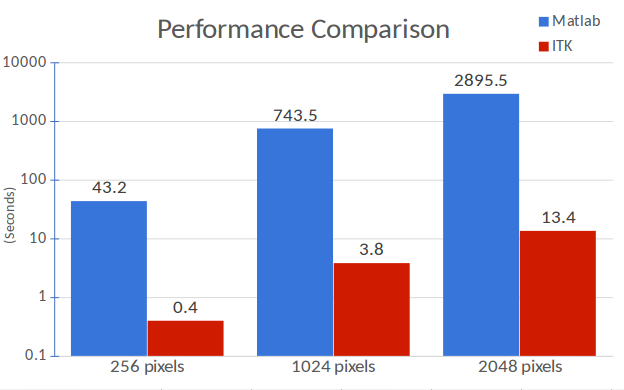
\includegraphics[height=0.9\textheight]{./figures/TextureFeaturesPerformanceComparison.png}
\end{frame}

\begin{frame}{Open Source Development}
  \begin{columns}[onlytextwidth]
    \column{0.80\textwidth}
    \metroset{block=fill}
    \begin{block}{All analysis filters were implemented as part of \textbf{ITK}, the Insight Toolkit:}
    \begin{itemize} \itemsep1.0em
      \item High performance, greatly reducing computational time in texture analysis.
      \item Able to compute 3D maps of multidimensional features
    \end{itemize}
  \end{block}
    \column{0.20\textwidth}
    \centering
    
\includegraphics[width=0.8\textwidth]{./logos/logo_ITK.png}
  \end{columns}
  \vspace{0.2cm}
  \begin{columns}[onlytextwidth]
    \column{0.80\textwidth}
    \metroset{block=fill}
    \begin{block}{\textbf{Python} packages available for Windows, Mac and Linux}
    % \noindent \textbf{Python} packages available for Windows, Mac and Linux
      \centering
      pip install itk-texturefeatures itk-bonemorphometry
  \end{block}
    \column{0.20\textwidth}
    \centering
    
\includegraphics[width=0.99\textwidth]{./logos/logo_python.png}
  \end{columns}
  \vspace{0.2cm}
  \begin{columns}[onlytextwidth]
    \column{0.80\textwidth}
    \metroset{block=fill}
    \begin{block}{Graphical interface in 3DSlicer: Bone Texture Extension}
    \end{block}
    \column{0.20\textwidth}
    \centering
    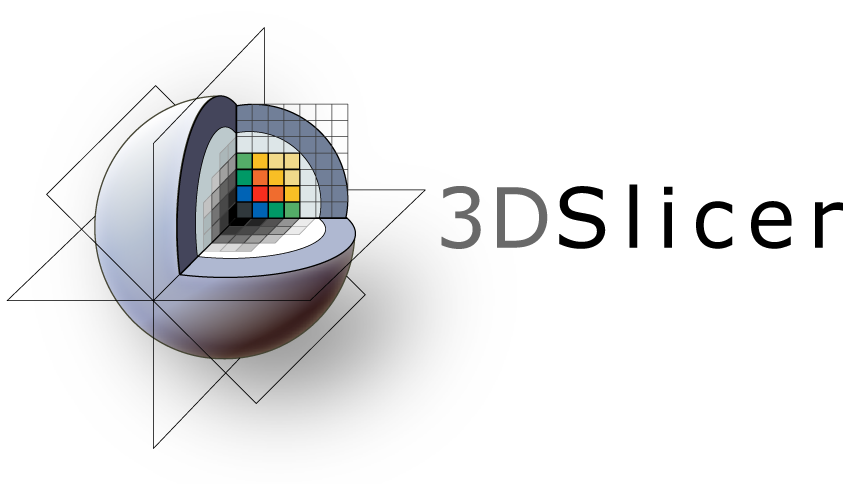
\includegraphics[width=0.9\textwidth]{./logos/logo_slicer_horizontal.png}
  \end{columns}
\end{frame}

{
\setbeamercolor{background canvas}{bg=kitwarewhite}
\begin{frame}{Medical Computing}
    \centering
    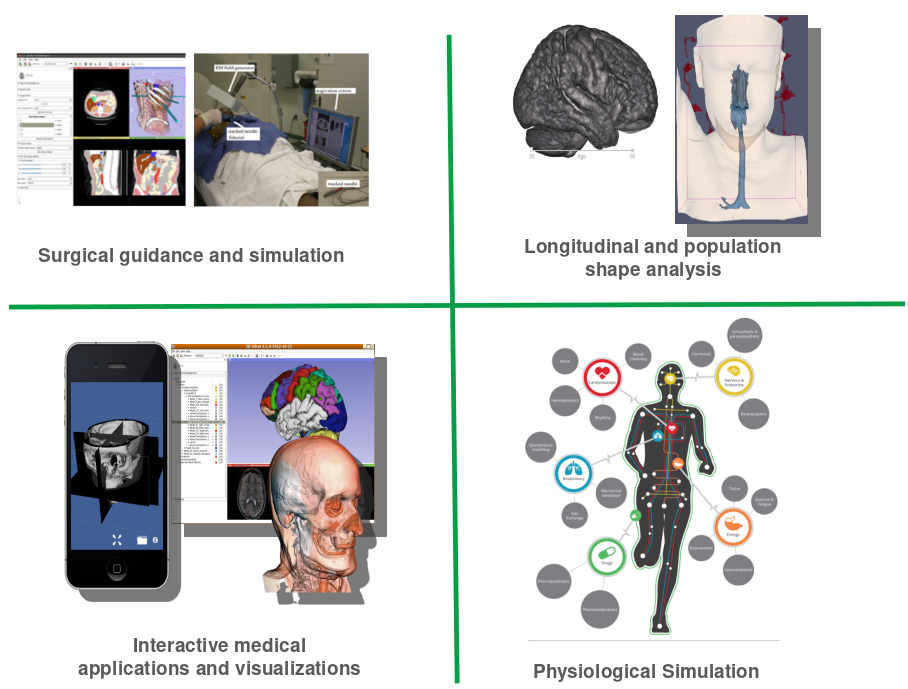
\includegraphics[height=0.9\textheight]{./logos/kitware_medical.png}
\end{frame}
}

\begin{frame}[standout]
  \centering
  {\huge Thanks!}\\
  pablo.hernandez@kitware.com\\
  kitware@kitware.com
  \vspace{1cm}
  % {\Huge Questions?}\\
\end{frame}

\appendix

{
\setbeamercolor{background canvas}{bg=kitwarewhite}
\begin{frame}[fragile]{GLCM Matrices}
  \centering
  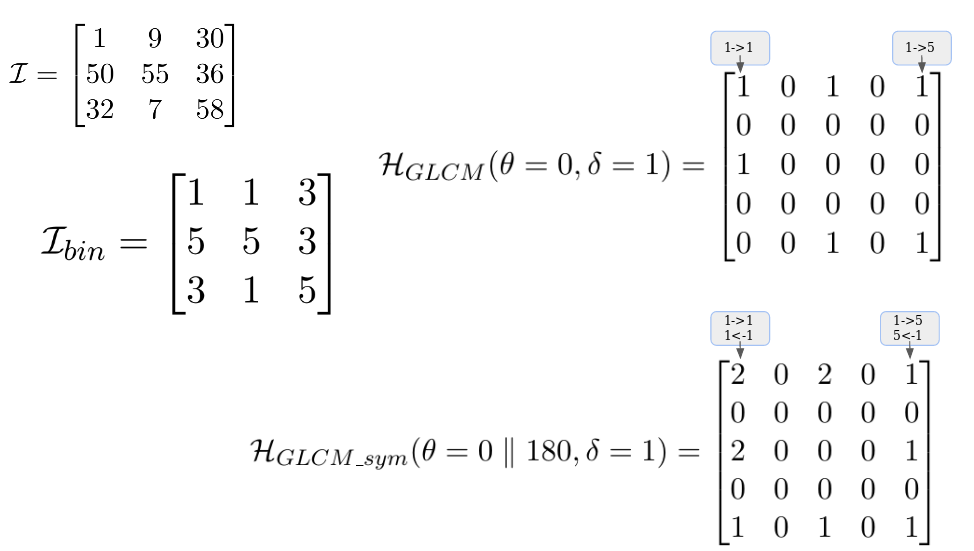
\includegraphics[width=0.9\textwidth]{./figures/GLCM_matrices.png}
\end{frame}

\begin{frame}[fragile]{GLRLM Matrices}
  \centering
  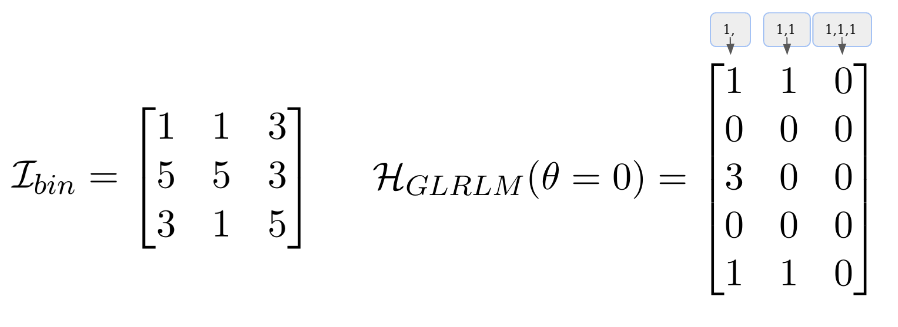
\includegraphics[width=0.9\textwidth]{./figures/GLRLM_matrices.png}
\end{frame}
}


\begin{frame}[allowframebreaks]{References}

  \bibliography{references}
  \bibliographystyle{abbrv}

\end{frame}


\end{document}

